\subsubsection{26.02.15}

\begin{enumerate}
	\item Time of beginning and ending of meeting:
	16:00 - 22:30
	\item Purposes of meeting:
	\begin{enumerate}
		\item To replace blades on the gripper for balls.
		
		\item To make the ramp for balls that fixed stationary.
	  
    \end{enumerate}
   
	\item Work that has been done:
	\begin{enumerate}
		 
		 \item It was decided to make blades by pieces of plastic bottle.
		 
		 \item It was found that when robot moves with raised lift small balls gets under the bucket. It prevents to lowering of the bucket. This was because the ramp for balls was fixed on the bucket. So it was decided to install the ramp stationary.
		 
		 \item It was made cardboard layout of the ramp. It was decided to fix the ramp on the slopes. 
		 		         \begin{figure}[H]
		 		         	\begin{minipage}[h]{0.2\linewidth}
		 		         		\center  
		 		         	\end{minipage}
		 		         	\begin{minipage}[h]{0.6\linewidth}
		 		         		\center{
\includegraphics[scale=0.07]{days/26.02.15/images/02}}
		 		         		\caption{Cardboard layout of the ramp}
		 		         	\end{minipage}
		 		         \end{figure}
		 
		 \item It was made the ramp of galvanized steel.
		 		         \begin{figure}[H]
		 		         	\begin{minipage}[h]{0.15\linewidth}
		 		         		\center  
		 		         	\end{minipage}
		 		         	\begin{minipage}[h]{0.6\linewidth}
		 		         		\center{
\includegraphics[scale=0.07]{days/26.02.15/images/03}}
		 		         		\caption{Steel ramp}
		 		         	\end{minipage}
		 		         \end{figure}		 
		 
		 
		 \item The ramp was tested and it was estimated optimal distance between the gripper for balls and ramp.
		 
		 \item It was found that when two balls gets into the gripper they stuck because they can't to pass between the slopes. So it was decided to cut one side of the blades of gripper. So the gripper capture one ball stronger than the second. Firstly the ball that captures by longer side of the blade gets into the bucket. When there is only one ball in the gripper it can to capture ball without problems.
		 		         \begin{figure}[H]
		 		         	\begin{minipage}[h]{0.2\linewidth}
		 		         		\center  
		 		         	\end{minipage}
		 		         	\begin{minipage}[h]{0.6\linewidth}
		 		         		\center{
\includegraphics[scale=0.1]{days/26.02.15/images/04}}
		 		         		\caption{Blades were cut}
		 		         	\end{minipage}
		 		         \end{figure}		 
		 
		 \item It was carried out training. During the training there was a problem that motors didn't work but servos and Lego motors worked. When we turned off the power and then turned on it this problem was solved. But if it will happen during the match we'll can't to do it. So it was elaborated mechanism that turns by Lego motor and press the button of power. It will need to connect two buttons one - for Samantha-module and the second - for controllers. This mechanism will press the second button. So the robot will not disconnect from the field control system. Also it will be more comfortable turn off the power from joystick. In addition we'll can turn off the power between autonomous and tele op period. So our battery will not discharge.
		 
		 \item The problem was that the balls can stuck in the bucket when it overturned. So it was decided to make asymmetrical bucket.
		         \begin{figure}[H]
		         	\begin{minipage}[h]{0.2\linewidth}
		         		\center  
		         	\end{minipage}
		         	\begin{minipage}[h]{0.6\linewidth}
		         		\center{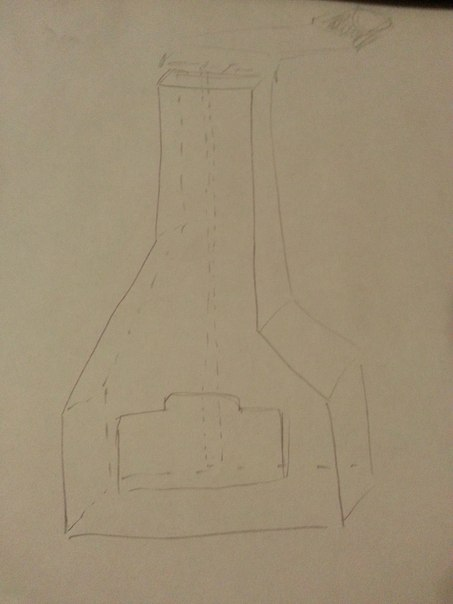
\includegraphics[scale=0.35]{days/26.02.15/images/01}}
		         		\caption{The idea of the new bucket}
		         	\end{minipage}
		         \end{figure}
		 
		 \item The blades of additional gripper were cut so that they doesn't hook the slopes when they under the load.
	      
    \end{enumerate}
    
	\item Result: 
	\begin{enumerate}
	  \item They were made new blades for gripper.		
		
	  \item It was projected new ramp for balls.
	  
	  \item The gripper for balls was improved.
	  
	  \item It was invented the idea of the automatical button of power.
      
      \item The blades on additional grippers for balls were cut so that they doesn't hook the slopes.
    \end{enumerate}
    
	\item Tasks for the next meetings:
	\begin{enumerate}
		\item To make a new bucket.
		
		\item To fix the ramp.
	  
    \end{enumerate}     
\end{enumerate}
\fillpage